% Figure 1: two-panel study overview, laid out flat and wide to keep its height
% inside the 5-page budget.
%   (a) Modality 1 development pipeline (QM9, 3D molecular coordinates)
%   (b) transfer of the same controller to Modality 2 (DNA, probability simplex)
%
% Keying convention, restated in the caption:
%   trainedbox = trained by us; frozenbox = trained by us, frozen at sampling;
%   pretrainbox = external pretrained, frozen; innovbox = changed by the innovation.
%
% Compile standalone:  pdflatex overview.tex   (from paper/figs/)
\documentclass[border=2pt]{standalone}
\usepackage{tikz}
\usepackage{amsmath}
\usepackage{amssymb}
\usetikzlibrary{arrows.meta,positioning,fit,backgrounds,calc}

\definecolor{cTrain}{HTML}{1F5FA9}
\definecolor{cFrozen}{HTML}{2F6B4F}
\definecolor{cPre}{HTML}{8A6D3B}
\definecolor{cInnov}{HTML}{B3261E}
\definecolor{cPanel}{HTML}{F6F7F9}

\begin{document}
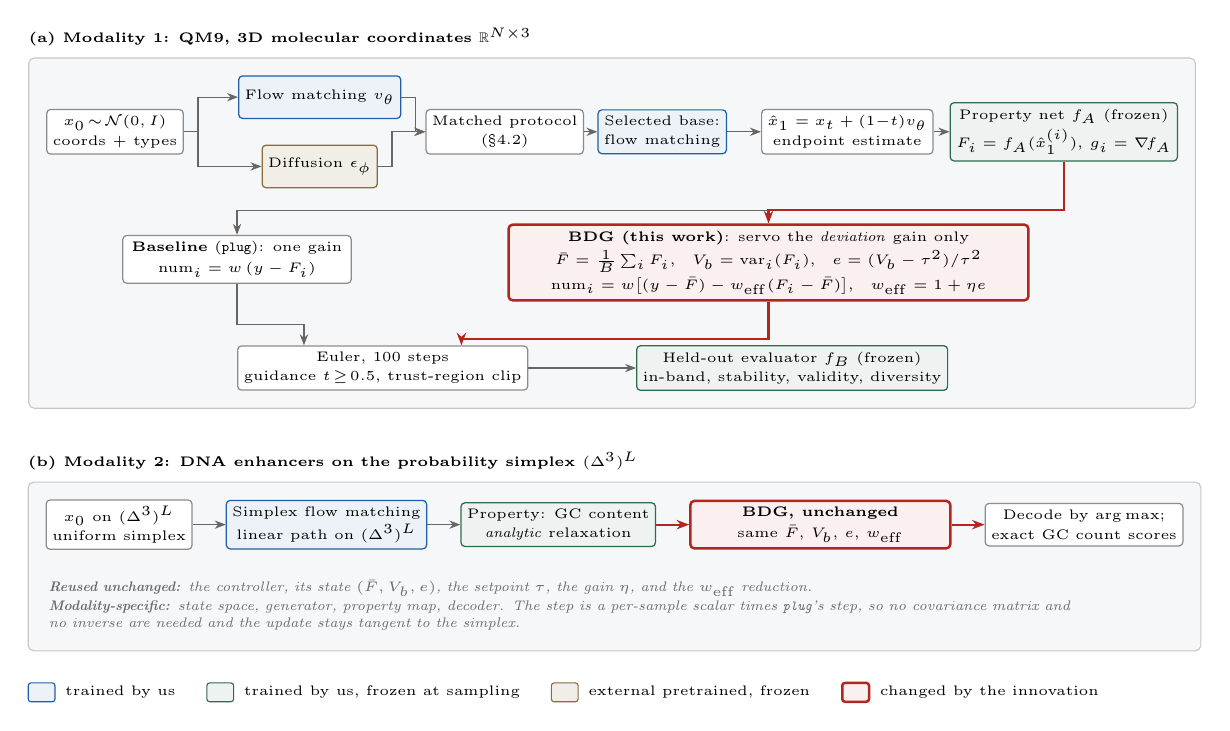
\begin{tikzpicture}[
  font=\tiny,
  box/.style={draw,rounded corners=1.4pt,align=center,inner sep=2.2pt,
              minimum height=5.4mm,line width=0.45pt},
  trainedbox/.style={box,draw=cTrain,fill=cTrain!8},
  frozenbox/.style={box,draw=cFrozen,fill=cFrozen!8},
  pretrainbox/.style={box,draw=cPre,fill=cPre!12},
  innovbox/.style={box,draw=cInnov,fill=cInnov!7,line width=0.9pt},
  plainbox/.style={box,draw=black!45,fill=white},
  ar/.style={-{Stealth[length=1.4mm]},draw=black!60,line width=0.45pt},
  arh/.style={-{Stealth[length=1.6mm]},draw=cInnov,line width=0.75pt},
  note/.style={font=\tiny\itshape,text=black!58,align=left,inner sep=1pt},
  panel/.style={draw=black!22,rounded corners=2pt,fill=cPanel,inner sep=2.2mm},
  ttl/.style={font=\tiny\bfseries,anchor=west,inner sep=0pt},
]

%% ===== PANEL (a), row 1: base-model selection, then the guidance inputs =====
\node[plainbox]    at (0    , 0    ) (x0a)  {$x_0\!\sim\!\mathcal{N}(0,I)$\\[1pt]coords $+$ types};
\node[trainedbox]  at (2.60 , 0.44 ) (fm)   {Flow matching $v_\theta$};
\node[pretrainbox] at (2.60 ,-0.44 ) (dm)   {Diffusion $\epsilon_\phi$};
\node[plainbox]    at (4.95 , 0    ) (sel)  {Matched protocol\\[1pt](\S4.2)};
\node[trainedbox]  at (6.95 , 0    ) (base) {Selected base:\\[1pt]flow matching};
\node[plainbox]    at (9.30 , 0    ) (mhat) {$\hat{x}_1 = x_t + (1{-}t)v_\theta$\\[1pt]endpoint estimate};
\node[frozenbox]   at (12.05, 0    ) (fa)   {Property net $f_A$ (frozen)\\[1pt]$F_i=f_A(\hat{x}_1^{(i)})$, $g_i=\nabla\! f_A$};

\draw[ar] (x0a.east) -- ++(0.18,0) |- (fm.west);
\draw[ar] (x0a.east) -- ++(0.18,0) |- (dm.west);
\draw[ar] (fm.east)  -- ++(0.18,0) |- (sel.west);
\draw[ar] (dm.east)  -- ++(0.18,0) |- (sel.west);
\draw[ar] (sel.east)  -- (base.west);
\draw[ar] (base.east) -- (mhat.west);
\draw[ar] (mhat.east) -- (fa.west);

%% ===== PANEL (a), row 2: the two guidance rules the paper compares =========
\node[plainbox,minimum width=2.9cm] at (1.55,-1.62) (plug)
  {\textbf{Baseline} (\texttt{plug}): one gain\\[1.5pt]
   $\mathrm{num}_i = w\,(y-F_i)$};
\node[innovbox,minimum width=6.6cm] at (8.30,-1.66) (bdg)
  {\textbf{BDG (this work)}: servo the \emph{deviation} gain only\\[1pt]
   $\bar F=\tfrac1B\sum_i F_i$,\;\; $V_b=\mathrm{var}_i(F_i)$,\;\;
   $e=(V_b-\tau^{2})/\tau^{2}$\\[1pt]
   $\mathrm{num}_i = w\big[(y-\bar F)-w_{\mathrm{eff}}(F_i-\bar F)\big]$,\;\;
   $w_{\mathrm{eff}}=1+\eta e$};

\draw[ar]  (fa.south) -- ++(0,-0.62) -| (plug.north);
\draw[arh] (fa.south) -- ++(0,-0.62) -| (bdg.north);

%% ===== PANEL (a), row 3: sampler and scoring ===============================
\node[plainbox]  at (3.40,-3.00) (samp) {Euler, 100 steps\\[1pt]guidance $t\!\ge\!0.5$, trust-region clip};
\node[frozenbox] at (8.60,-3.00) (fb)   {Held-out evaluator $f_B$ (frozen)\\[1pt]in-band, stability, validity, diversity};

\draw[ar]  (plug.south) -- ++(0,-0.52) -| ([xshift=-1.0cm]samp.north);
\draw[arh] (bdg.south)  -- ++(0,-0.48) -| ([xshift=1.0cm]samp.north);
\draw[ar]  (samp.east)  -- (fb.west);

\begin{scope}[on background layer]
  \node[panel,fit=(x0a)(fm)(dm)(sel)(base)(mhat)(fa)(samp)(fb)(plug)(bdg)] (pa) {};
\end{scope}
\node[ttl] at ([yshift=2.6mm]pa.north west)
  {(a) Modality 1: QM9, 3D molecular coordinates $\mathbb{R}^{N\times3}$};

%% ================================ PANEL (b) ==============================
\coordinate (bo) at ([yshift=-1.15cm]pa.south west);

\node[plainbox,anchor=north west]  at ($(bo)+(0.22,0)$)      (x0b) {$x_0$ on $(\Delta^{3})^{L}$\\[1pt]uniform simplex};
\node[trainedbox,anchor=west]      at ($(x0b.east)+(0.42,0)$) (sfm) {Simplex flow matching\\[1pt]linear path on $(\Delta^{3})^{L}$};
\node[frozenbox,anchor=west]       at ($(sfm.east)+(0.42,0)$) (gc)  {Property: GC content\\[1pt]\emph{analytic} relaxation};
\node[innovbox,anchor=west,minimum width=3.3cm] at ($(gc.east)+(0.42,0)$) (bdg2)
  {\textbf{BDG, unchanged}\\[1.5pt]same $\bar F$, $V_b$, $e$, $w_{\mathrm{eff}}$};
\node[plainbox,anchor=west]        at ($(bdg2.east)+(0.42,0)$) (dec) {Decode by $\arg\max$;\\[1pt]exact GC count scores};

\draw[ar]  (x0b.east) -- (sfm.west);
\draw[ar]  (sfm.east) -- (gc.west);
\draw[arh] (gc.east)  -- (bdg2.west);
\draw[arh] (bdg2.east) -- (dec.west);

\node[note,anchor=north west,text width=13.2cm] at ($(x0b.south west)+(0,-0.34)$) (chg)
  {\textbf{Reused unchanged:} the controller, its state $(\bar F, V_b, e)$, the setpoint $\tau$, the gain $\eta$, and the $w_{\mathrm{eff}}$ reduction.\\[1pt]
   \textbf{Modality-specific:} state space, generator, property map, decoder. The step is a per-sample scalar times \texttt{plug}'s step, so no covariance matrix and no inverse are needed and the update stays tangent to the simplex.};

\begin{scope}[on background layer]
  \node[panel,fit=(x0b)(sfm)(gc)(bdg2)(dec)(chg)] (pb) {};
\end{scope}
\node[ttl] at ([yshift=2.6mm]pb.north west)
  {(b) Modality 2: DNA enhancers on the probability simplex $(\Delta^{3})^{L}$};

%% ================================= LEGEND ================================
\begin{scope}[shift={([yshift=-0.52cm]pb.south west)},font=\tiny]
  \node[draw=cTrain,fill=cTrain!8,rounded corners=1pt,minimum height=2.4mm,
        minimum width=3.4mm,anchor=west] at (0,0) (k1) {};
  \node[anchor=west,inner sep=1pt] at (k1.east) (kt1) {\ trained by us};
  \node[draw=cFrozen,fill=cFrozen!8,rounded corners=1pt,minimum height=2.4mm,
        minimum width=3.4mm,anchor=west] at ([xshift=3.5mm]kt1.east) (k2) {};
  \node[anchor=west,inner sep=1pt] at (k2.east) (kt2) {\ trained by us, frozen at sampling};
  \node[draw=cPre,fill=cPre!12,rounded corners=1pt,minimum height=2.4mm,
        minimum width=3.4mm,anchor=west] at ([xshift=3.5mm]kt2.east) (k3) {};
  \node[anchor=west,inner sep=1pt] at (k3.east) (kt3) {\ external pretrained, frozen};
  \node[draw=cInnov,fill=cInnov!7,rounded corners=1pt,line width=0.9pt,
        minimum height=2.4mm,minimum width=3.4mm,anchor=west] at ([xshift=3.5mm]kt3.east) (k4) {};
  \node[anchor=west,inner sep=1pt] at (k4.east) {\ changed by the innovation};
\end{scope}

\end{tikzpicture}
\end{document}
